\section{Introduction and Background}

This document describes the Risk \& Opportunity Management Plan used to identify, assess, respond to, and manage risks and opportunities associated with the technical, cost and schedule aspects for the Vera C.\ Rubin Observatory throughout the operation of the Legacy Survey of Space and Time (LSST).
The Rubin Observatory Risk \& Opportunity Management Plan recognizes the benefits of managing uncertainty during operations in a holistic and systematic manner.

The Risk \& Opportunity Management Plan is one plan in a group of Rubin Observatory Operations plans that collectively define a comprehensive approach to managing risk, and opportunity, which are collectively known as approaches to making decisions under conditions of uncertainty.
Risk of harm to personnel and equipment is the focus of the Rubin Observatory Safety Policy, \citeds{RDO-015}.
Further aspects of risk and safety management are codified under the NSF (National Science Foundation) NOIRLab and the Department of Energy (DOE) SLAC Laboratory (SLAC National Accelerator Laboratory) documents where appropriate. 
Additionally and were applicable,  risk, safety, and hazard analysis plans are adopted for Rubin Observatory Operations from the Rubin Observatory Construction Project .

The key aspects of the Risk \& Opportunity Management Plan are:
\begin{itemize}
	\item A standard methodology to identify and assess major risks and opportunities associated with Operations work breakdown structure (WBS) elements and operations functions from the Operations Plan.

	\item A continuous process to review and re-assess current risks and opportunities on a quarterly or semi-annual basis and address new risks and opportunities as they emerge.
	
	\item Common techniques for assignment of budget and schedule for the anticipated response in the event of a realized risk.
	
	\item An approach and tool to measure and compare to contingency levels, the remaining major risk exposure across operation.
	
	\item A single dynamic and interactive system to inform management, to support communication across operations, to facilitate and encourage regular participation of team members, and to produce standard reporting and tracking features.
\end{itemize}


\subsection{Risk Management Process Overview}

The risk management process is a continuous and proactive approach to keeping risk at an acceptable level through awareness, tracking, and response handling.
The Rubin Observatory Risk Management process is an event-centric approach.
It is characterized by the identification of events that may occur in the future with resulting negative or positive consequences for operations.
There are different types of risk associated with Rubin Observatory Operations:
\begin{itemize}
\item Technical Risk, consisting of the risk of not meeting survey performance requirements or deliverables;
\item Cost Risk, consisting of the risk that the available budget will be insufficient to cover the scope of operations;
\item Schedule Risk, consisting of the risk that the survey will fail to meet scheduled milestones; and,
\item a related category of risk is called Programmatic Risk, which is risk produced by events that are beyond the control of the operations management team, where programmatic Risk can be a source of risk in any of the other three risk categories. 
\end{itemize}

In transitioning from the construction phase to operations, the operations team will consult with the Rubin Observatory  project to understand any project risks that might transfer to operations or (more likely) evolve into operations risks.
During the pre-operations phase, which occurs in parallel with the project integration and commissioning phases, the operations team will work closely with the project team to understand all risks, safety plans, and hazards and adapt, revise, and establish analogous processes, procedures, and policies.
This transition will take place from the beginning of pre-operations and be completed no later than the Operations Readiness Review (ORR), which marks formal handover of the Rubin Observatory system from the project to the operations team.

\subsection{Risk Management Tools}

Rubin Observatory Operations will follow the NOIRLab model, shown Figure \ref{fig:NOIRLab-risk-model} for managing its risks and opportunities. 
The Alcea Tracking Solutions (ATS) software tool for risk management, which has been adopted by NOIRLab, will used by Rubin.   
The user guide for the ATS  tool is found in \citeds{RTN-051}.

In addition to this, Rubin may choose to implement additional tools on top of the Alcea tool to better integrate the process of risk and opportunity management into the Rubin workflow. 
Any additional such tools developed by Rubin for managing risks will be added to this document as they are developed. 
 
All risks are reported to AURA and SLAC management, as well as NSF through NOIRLab quarterly reports.

\begin{figure}[t]
\caption{NOIRLab Risk Management Model.}
\centering
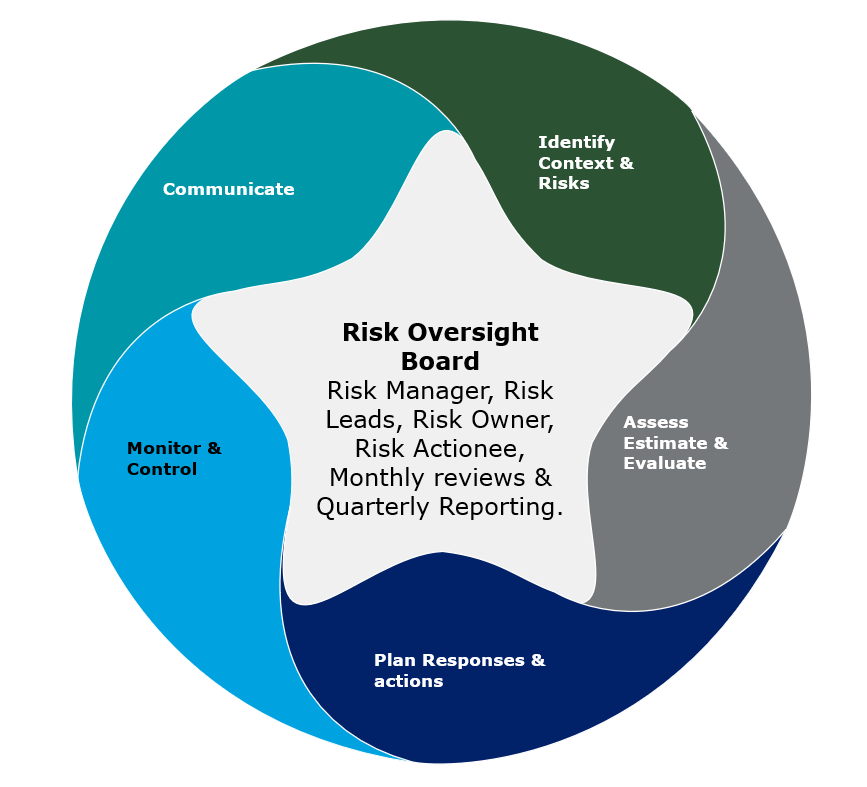
\includegraphics[width=\textwidth]{NOIRLab-risk-model-temp}
\label{fig:NOIRLab-risk-model}
\end{figure}


\subsection{Roles and Responsibilities}

The Rubin Observatory Risk \& Opportunity Board (RROB) serves as the managing group for the Risk \& Opportunity Management Plan.
The RROB is managed by the System Performance (SP) Department.

The \textbf{Rubin Observatory Operations Director} has overall responsibility for managing and controlling operations risks.
The Director will work with the senior managers to review and assess current risks on a quarterly basis.
The Director will also approve all new risks (or delegate this responsibility as appropriate to another operations manager) in coordination with the RROB.

The \textbf{Rubin Observatory Executive Council} is the group of operations management and leadership staff charged with reviewing the risk registry, evaluating the risk and opportunity assessments, collaborating on risk handling options, and developing implementation recommendations, which are forwarded to the Director of operations.
The Executive Council consists of the Associate Directors (ADs) and Deputy Directors as well as other operations staff.
It is expected that the head of safety for NOIRLab will meet with the Executive Council to regularly review risks.

